\documentclass[conference]{IEEEtran}

\usepackage[utf8]{inputenc}
\usepackage[T1]{fontenc}
\usepackage[english]{babel}

% Graphics
\usepackage{graphicx, float, subfigure, blindtext}

\newcommand\IEEEhyperrefsetup{
bookmarks=true,bookmarksnumbered=true,%
colorlinks=true,linkcolor={black},citecolor={black},urlcolor={black}%
}

% Preferred hyperref setup, Michael Shell
\usepackage[\IEEEhyperrefsetup, pdftex]{hyperref}

% Maths
\usepackage{mathtools}

% These packages must be at the end
\usepackage[nolist,nohyperlinks]{acronym}
\usepackage{cleveref}
\graphicspath{{images/}}

% Remove section first paragraph indent
\usepackage{titlesec}
\titlespacing*{\section}{0pt}{*1}{*1}
\titlespacing*{\subsection}{0pt}{*1}{*1}
\renewcommand{\thesubsubsection}{\arabic{subsubsection}}
\titleformat{\subsubsection}[runin]{\itshape}{\thesubsubsection)}{1em}{}[:]
\titlespacing*{\subsubsection}{\parindent}{0pt}{*1}

% Include authors 
\author{\IEEEauthorblockN{ %
Adrian Swande\IEEEauthorrefmark{1},
Oskar Frej\IEEEauthorrefmark{2},
Gustav Samuelson\IEEEauthorrefmark{3},
Ivan Blazanovic\IEEEauthorrefmark{4},
Lukas Bonkowski\IEEEauthorrefmark{5}
}
\IEEEauthorblockA{
School of Innovation, Design and Engineering, M.Sc.Eng Robotics\\
Mälardalens University, Västerås, Sweden\\
Email:
\IEEEauthorrefmark{1}ase22003@student.mdu.se,
\IEEEauthorrefmark{1}ofj22001@student.mdu.se,
\IEEEauthorrefmark{1}gsn22003@student.mdu.se,
\IEEEauthorrefmark{1}...@student.mdu.se,
\IEEEauthorrefmark{1}...@student.mdu.se,
}}

% ACRONYMS: \acrodef{acronym}[short name]{full name}
\acrodef{svm}[SVM]{Support Vector Machine}

% The report title.
\title{Robocup SLL}
% Document begins here
\begin{document}
% Create the title.
\maketitle
% Example sections, name them
% according to specific needs.
\begin{abstract}
An abstract should summarize the work in brief. 

\end{abstract}
\begin{center}
\begin{IEEEkeywords}
AI, Autonomous Robots, RoboCup, Soccer
\end{IEEEkeywords}
\end{center}

\section{Introduction}
\label{section:intro}

The RoboCup \cite{RoboCupSSL} is a tournament where different teams compete against each other with soccer playing robots. The RoboCup Federation arranges several types of leagues where every league uses different types of robots in different shapes and sizes. Overall, this tournament aims to advance in the scientific field of mobile robots. 
This project will focus on the Small Size League (SSL), division B in particular. In the SSL division B teams compete in 6 vs 6 matches of two halves where each half is five minutes long with a five-minute pause in between. The robots are constrained to certain physical dimensions according to the rules (the robots need to fit inside a cylinder of 0.18 meters width and 0.15 meters height) and the robots are built by the members of each team. The playing field is 10.4 times 7.4 meters with a playing area of 9 times 6 meters and the game is played with an orange golf ball. The rules of this league are similar to regular soccer but with several modifications. For example the rules include yellow and red cards, freekicks and penalties but also rules like maximum shooting speed and maximum dribbling length. 
The aim of this project is to develop a system that works well in simulation. That will be done by creating an AI system that can coordinate all six robots, handle the ball, score goals and defend against the opponents. In the long term the models we develop could be further developed and used in other works related to both RoboCup and other areas. In this paper we aim to answer the question of how transferable policies trained in simpler, more abstracted simulators like \acronym{VMAS} are to more accurate simulators such as grSim, and at which level of the hierarchal AI model.

\section{Method}
\label{section:method}
In this section, the method used to find an answer to the research questions should be presented. 

If this report presents results from a literature search, this means providing sufficient information for allowing someone else to repeat the literature search and compare the results. I.e., a search using the phrases a, b, and c, was made in database x, y and z on the date Month Date, Year (e.g., July 31st, 2021). The search resulted in x hits. Then, information on how you chose which works to include in this report should be provided. The references should be used for answering your research questions.

If the work reports on an experiment, this part should provide information about the experimental setup, how the experiment was conducted, how data was collected and analyzed etc. Motivate methodological choices through references. Also an experiment should be presented with sufficient detail such that it can be repeated by someone else.
\section{Results}
\label{section:results}

\subsection{rcssserver}
The use of rcssserver led to us achieving a basic but working simulation that was used to perform the training for the genetic algorithm.

\subsection{Genetic algorithm}
In figures 3 and 4 are shown the results of the evolution of the configuration vector \(c\in\mathcal{C}\) by means of the genetic algorithom described in \textit{Method}. The best individual after ca. 30 generations was tested against best programmer-defined configuration in a 1 vs. 1 scenario where they were instructed to move the ball into the other player's goal. If none of the players had managed to score a goal after 60 seconds, the game was counted as a draw. The results of 25 games is shown in figure 5.

\begin{figure}[tbp]
\centering
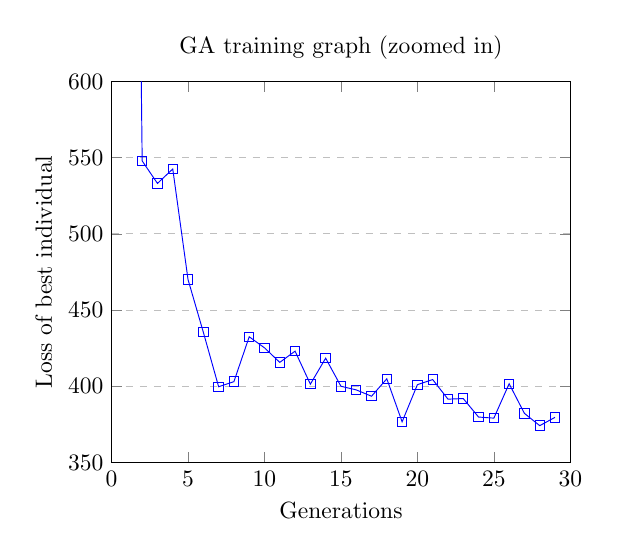
\begin{tikzpicture}[scale=0.85]
\begin{axis}[
    title={GA training graph (zoomed in)},
    xlabel={Generations},
    ylabel={Loss of best individual},
    xmin=0, xmax=30,
    ymin=350, ymax=600,
    xtick={0,5,10,15,20,25,30},
    ytick={300,350,400,450,500,550,600,650,700,750,800,850,900,950,
    1000,1050,1100,1150,1200,1250,1300,1350,1400,1450,1500},
    %ytick={300,400,500,600,700,800,900,1000,1100,1200,1300,1400,1500},
    legend pos=north west,
    ymajorgrids=true,
    grid style=dashed,
]

\addplot[
    color=blue,
    mark=square,
    ]
    coordinates {
(1,1436.1875)(2,547.875)(3,533.125)(4,542.59375)(5,470.0)(6,435.5)(7,399.71875)(8,403.0625)(9,432.5)(10,425.25)(11,415.71875)(12,423.0625)(13,401.40625)(14,418.46875)(15,400.03125)(16,397.65625)(17,393.5)(18,404.9375)(19,376.71875)(20,401.0625)(21,404.4375)(22,391.59375)(23,391.96875)(24,379.84375)(25,379.125)(26,401.6875)(27,382.25)(28,374.1875)(29,379.65625)
    };


\end{axis}
\end{tikzpicture}
	\caption{Graph showing the loss function of the best individual through generations.}
\end{figure}



\begin{figure}[h]
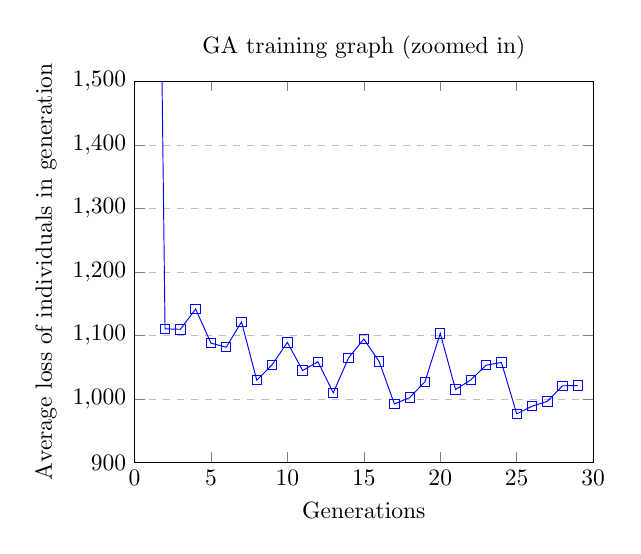
\begin{tikzpicture}[scale=0.85]
\begin{axis}[
    title={GA training graph (zoomed in)},
    xlabel={Generations},
    ylabel={Average loss of individuals in generation},
    xmin=0, xmax=30,
    ymin=900, ymax=1500,
    xtick={0,5,10,15,20,25,30},
    %ytick={300,350,400,450,500,550,600,650,700,750,800,850,900,950,
    %1000,1050,1100,1150,1200,1250,1300,1350,1400,1450,1500},
    %ytick={500,1000,1500,2000,2500,3000,3500},
    ytick={900,1000,1100,1200,1300,1400,1500},
    legend pos=north west,
    ymajorgrids=true,
    grid style=dashed,
]

\addplot[
    color=blue,
    mark=square,
    ]
    coordinates {
(1,3098.46875)(2,1110.4375)(3,1109.7916666666667)(4,1141.7135416666667)(5,1087.9895833333333)(6,1081.5625)(7,1121.390625)(8,1029.5989583333333)(9,1053.84375)(10,1089.21875)(11,1044.875)(12,1058.734375)(13,1009.7395833333334)(14,1064.5989583333333)(15,1094.4947916666667)(16,1059.1302083333333)(17,992.2916666666666)(18,1002.25)(19,1027.1927083333333)(20,1103.2864583333333)(21,1014.921875)(22,1030.1770833333333)(23,1053.2135416666667)(24,1057.5364583333333)(25,976.6666666666666)(26,988.5833333333334)(27,996.3333333333334)(28,1020.8177083333334)(29,1021.2708333333334)
    };


\end{axis}
\end{tikzpicture}
	\caption{Graph showing the mean value of the loss function for each individual through generations.}
\end{figure}

\begin{figure}[h]
\begin{tabular}{lllll}
\cline{1-3}
\multicolumn{1}{|l|}{GA wins}         & \multicolumn{1}{l|}{18} & \multicolumn{1}{l|}{72\%} &  &  \\ \cline{1-3}
\multicolumn{1}{|l|}{Programmer wins} & \multicolumn{1}{l|}{4}  & \multicolumn{1}{l|}{16\%} &  &  \\ \cline{1-3}
\multicolumn{1}{|l|}{Draws}           & \multicolumn{1}{l|}{3}  & \multicolumn{1}{l|}{12\%} &  &  \\ \cline{1-3}
\end{tabular}
		\caption{Results of GA-vs-programmer experiment shown in amount and percentage.}
\end{figure}

\subsection{rcssserver}
The use of rcssserver led to achieving a basic but working simulation that was used to perform the training for the genetic algorithm.

\subsection{Reinforcement Learning}
The experiments with reinforcement learning did not give the desired results.  
Even in basic scenarios, the agent was not able to score goals consistently.  
Training in a basic two-player setup did not show any coordinated and cooperative play between the two players.  
The players run towards the ball slowly and dribble towards the goal.  
Shooting was hard to replicate even in simplified scenarios.  

\subsection{Rule-Based System}
The best results were achieved when the blue agents utilized a Rule-Based System. When employing the Rule-Based System, 
the blue team consistently outperformed the hardcoded red team, winning every simulated match.

\section{Discussion}
\label{section:disc}

\subsection{Reinforcement Learning}
The results we achieved with applying PPO to our VMAS Robocup SSL setup were not as expected.
In this section, We will lay out why we think the results were unsatisfactory and what we could do differently to train our agent to achieve coordinated, cooperative play and, most importantly, score goals and defend effectively.

First and foremost, we would need to create a simulator where the basic mechanics work reliably. In particular, shooting and passing need improvement. Step-by-step debugging showed that these actions often require the robot to be in the exact right position and angle.

Once this is achieved, we also have lots of other ways we could improve our agent.

\subsubsection{Changing our low level skills}
Our agent selects from hard-coded low level skills. For the agent to behave as intended, these have to be carefully selected and implemented robustly.

\subsubsection{Reward shaping}
There is a lot of room for improvement through changing our reward function.
One aspect we haven't considered yet in our reward function is passing as a reward.
Previous work shows promise in rewarding successful passes, not being intercepted, and giving a negative reward for intercepted passes
(Wei, R., Ma, W., Yu, Z., Huang, W., \& Shan, S. SRC 2018 Team Description Paper).

With our centralized approach, we can design the reward function with the state and actions of all players, not just individuals.
More strategic behaviour could therefore be achieved by maintaining good spacing, occupying key positions, and setting up opportunities for passing and teamwork.
Rewards have to be considered carefully. Our shaped rewards must still align with our primary objectives:
\begin{itemize}
    \item Scoring goals
    \item Effective defense
\end{itemize}
so that agents do not focus too much on subgoals at the expense of overall team performance.

Due to our inconsistent results stemming from our core simulation issues, we did not include systematic evaluation and visualizations of agent performance.

In future work, once the simulation inconsistencies are addressed, we plan to implement more systematic evaluation of agent performance. This would include tracking and visualizing learning curves, episode rewards, and success rates for key behaviours such as scoring and passing. These evaluation methods are necessary for diagnosing problems and refining progress on agent results.

\section{Conclusion}

For VMAS we were able to create a custom environment made for
RoboCup SSL with working low-level skills. In that environment, we managed to train the agents to go to the
ball using reinforcement learning but unfortunately no
other training succeeded. For rcssserver, we managed to setup a working simulation environment, where we were able to create low-level skills and
coordinate them via a BT. We were able to tune these skills using
GA with positive results.

\section*{Acknowledgment}
The authors would like to thank ... for his/her/their help and support during the process of writing this paper. 
% Select the IEEEtran style
\bibliographystyle{IEEEtran}
% Include bibliography file
\bibliography{IEEEabrv,refs}
\end{document}